\subsubsection{Vận hành quầy và đồng bộ trạng thái}
\label{sec:staff-design}
Barista xử lý theo chuỗi PAID $\rightarrow$ PREPARING $\rightarrow$ READY $\rightarrow$ COMPLETED trên bảng bốn cột: chờ duyệt, đang pha, sẵn sàng và hoàn tất. Đơn PENDING/PAYMENT\_FAILED/CANCELLED không vào hàng đợi pha chế. Thao tác quầy chỉ đổi trạng thái phục vụ, không tạo Payment, giữ nguyên liệu hoặc cộng điểm lần nữa. Quyền BARISTA áp dụng ở backend như mục~\ref{sec:auth-design}.

findForStaff lấy mọi đơn đang xử lý theo createdAt/id tăng dần và tối đa 20 đơn hoàn tất gần nhất. Hai nhóm được đọc trong transaction RepeatableRead để tránh một đơn vừa chuyển COMPLETED bị mất hoặc lặp do đọc ở hai thời điểm khác nhau. Giới hạn 20 chỉ áp dụng nhóm hoàn tất, không cắt mất đơn đang chờ làm.

Đơn có yêu cầu đổi REQUESTED phải được duyệt/từ chối/rút trước khi bắt đầu pha. Khi quầy cập nhật thành công, backend commit rồi phát sự kiện orders.changed. Sự kiện chỉ báo có thay đổi, không mang thông tin đơn/tài khoản; client gọi lại API có xác thực và quyền đọc tương ứng. WebSocket là tín hiệu đồng bộ, còn database/API là nguồn trạng thái thật.

\begin{figure}[htbp]\centering
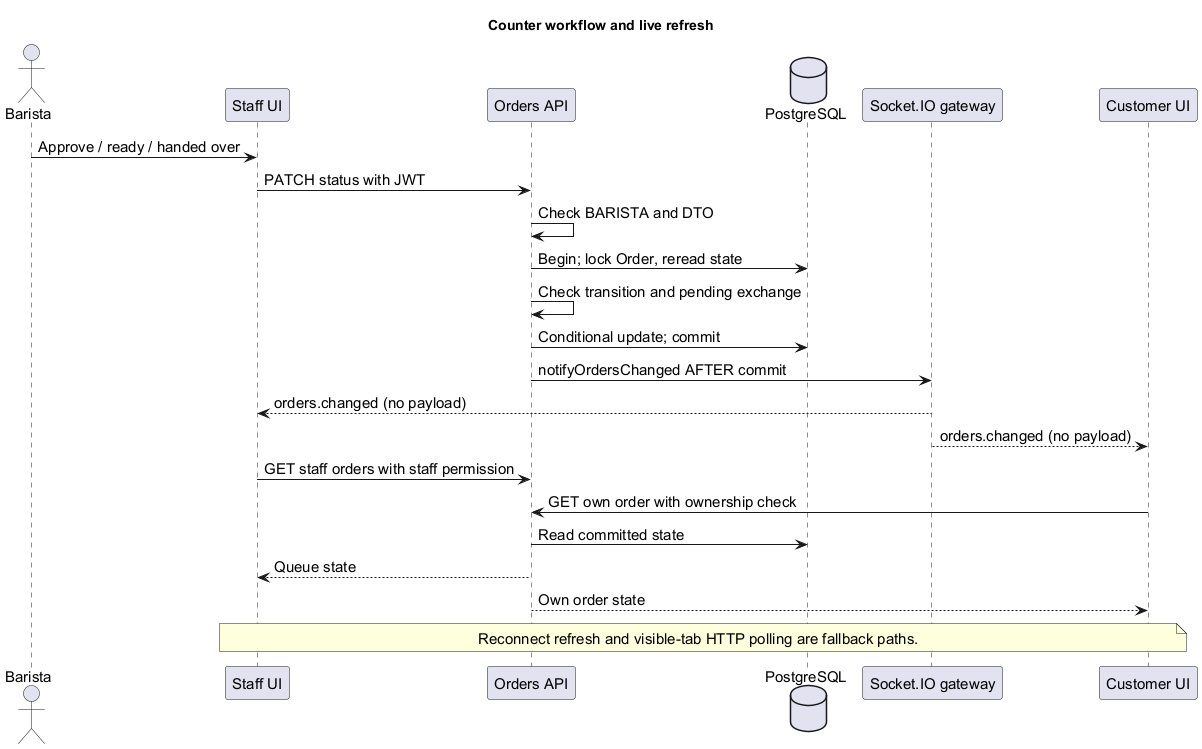
\includegraphics[width=\linewidth,height=.49\textheight,keepaspectratio]{assets/staff/staff-realtime.png}
\caption{Cập nhật trạng thái tại quầy, commit rồi thông báo để mỗi client đọc lại API được phép}
\end{figure}
